\chapter{Methodology}
\label{cha:methodology}
In this chapter we present the reader with a breakdown of tools and techniques used in experimental analysis. We partition our approach into three categories, each focused on addressing a particular section of our overarching hypothesis. We firstly discuss the implementation of our network simulation environment and list of produced tools in \cref{sec:Msimenvironment}. In this section we additionally cover the technical implementations of the network, probe paths, and other data structure choices. Secondly we explain our approach to testing the sub-hypothesis that network tomography enables inference of node level packet delay metrics within stochastically routing networks. We detail specifics of how we have applied network tomography and evaluated its accuracy w.r.t inferring node level metrics in \cref{sec:Mnetworkprobing}.\par
In \cref{sec:MNefidentification} we give an overview of our approach to determining router level nefarious hold probability in . In this analysis we identify a novel parametric relationship between router hold probability and packet delay. We then show how this relationship can be inverted to estimate router hold probability from packet delay. Thirdly in \cref{sec:Moptprobing} we then present the idea of the tomographic pipeline to segment the complex process of network tomography. We then cover our implementation of two optimisations to the tomographic pipeline using techniques introduced in \cref{cha:background}. Finally in \cref{sec:Mevaltechniques} we present methods we use for evaluating the significance of our findings and presenting results empirically.

\section{Simulation Environment and Tools}
\label{sec:Msimenvironment}

\section{Inferring Packet Delay Metrics}
\label{sec:Mnetworkprobing}
    To determine whether a router is behaving nefariously we must establish and verify a quantitative metric that is impacted by this nefarious behaviour. Using tomography we are able to observe end-to-end metrics, the additive metric of packet delay was an appealing option as we expect the nefarious delaying of routers to impact packet delay.
    
    Story Plan:
    \begin{itemize}
        \item Ability of packet delay metrics to detect nefarious behaviour in 'baseline' network
        \item Changing nefarious router within baseline
        \item Does Inference hold over variable network attributes?
        \begin{itemize}
            \item Router queue length
            \item Network background traffic
            \item Network topology
        \end{itemize}
        \item Testing variable queue length and background traffic in the baseline network
        \item Sigmoid curve from PDA being a likely candidate (as we want to infer when a router is very nefarious) warrants further investigation Need to mention Dogbox, TRF, and Levenberg–Marquardt.
        \item Determining relationship between PDA-holdprob curve and network attributes of queue length and background traffic.
        \begin{itemize}
            \item Curve fitting relationship using popular minimization algorithms avaliable in scipy: dogbox, trf and lm.
            \item Selected the best curve fitting minimization for use.
        \end{itemize}
        \item Generated network topologies - 50 ER and 50 BA with varying \# of routers from 30-100
        \item Varying queue length and background traffic in each of these generated configurations, measuring PDA.
        \item Real world topologies with varying \# of routers - testing impact of queue length and background traffic.
        \item Validate weather the sigmoid and network attributes hold over arbitrary generated and real world topologies.
    \end{itemize}
    
    \todo{Explain why the second order stat of variation is better for clock sync, but show accuracy issues vs first order average (reference results).}

    
\section{Identifying Nefarious Behaviour}
\label{sec:MNefidentification}
Todo:
\begin{itemize}
    \item Tomography as a linear system with a linear solution (note can include multiple routers in probe paths for identifiability just need to divide by the number of times it appears).
\end{itemize}

    \begin{mdframed}
    \textbf{NOTATION FOR PDV SECTION FORMALIZATION}:\\
    Probe path probabilities: Each probe packet is sent along a probe path $p$ with a probability of $\phi_p$, given there are multiple paths within any non-trivial model we represent them all as $\vec{\phi}=\forall p\in P^*, \phi_p$ where $|\vec{\phi}|=|P^*|$, $\phi_p \geq 0$ and $\sum_{p\in P^*}\phi_p = 1$
    
    The parameter vector $\vec{\theta}$ is the vector of length $|R|$ containing the parameter governing each $q\in Q$ where $ q_x \sim \theta_x$ or more formally $\vec{\theta}=\forall r\in R, \theta_r$.
    
    The vector $\vec{\psi}$ is the vector containing all proper path allocations/injection probabilities where $\psi_x$ is the allocation of probes to $p_x\in P^*$ 
    
    Let $f_{Q|\vec{\theta}}(q)$ represent the probability of observing the value $q$ from monitor-to-monitor probe path $p\in P^*$ given the node parameter $\theta_x$ governing $Q_x$.
    
    Note that we can represent a tomographic problem as a system of $P^*f'(\theta)=\mathcal{M}$ where $f'$ is a one-to-one correspondence function of $\theta$ and $\mathcal{M}$ is a matrix of monitor-to-monitor metrics we collect from our probing where $\mathcal{M}_p = (q_1,q_2,\ldots, q_n)$. For ease of notation let $|\mathcal{M}_p|$ be the number of metrics ($n$) we collect over path $p$. Note that for aggregation of measurements after collection $\forall p\in P^*, \forall r\in p, \mathcal{M}=\sum_{r\in p}\theta_r$.
    \end{mdframed}
    \todo{Integrate this into this section}

    To best utilise previous work on tomography we generalise our network as an $|\gls{routers}|\times|\gls{routers}|$ adjacent matrix where the $i$th$\times j$th entry is a 1 if router \emph{i} and \emph{j} are connected and a 0 otherwise. Such an adjacency matrix is often referred to in network science as a routing matrix, as both terms are appropriate depending on circumstance we will use them interchangeably. From this notation we are able to express the network shown in \cref{fig:6routersample} where $M=\{s_{0,0},s_{5,0}\}$ as the adjacency matrix $A$:
    
    \begin{figure}[H]
        \centering
        \tikzsetnextfilename{6routertopology}
        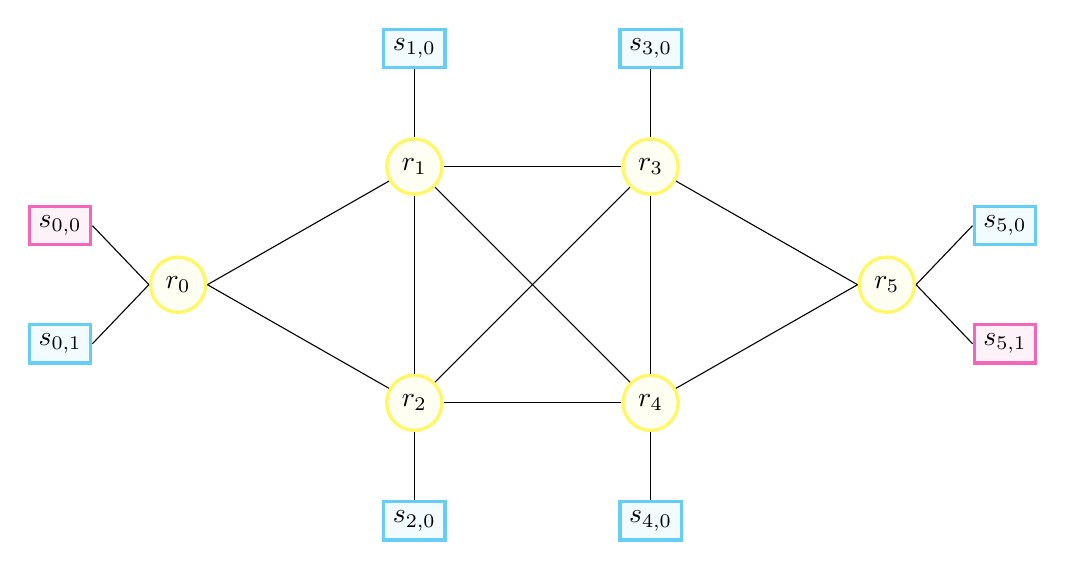
\begin{tikzpicture}[
            router/.style={circle, draw=yellow!60, fill=yellow!5, very thick, minimum size=3.5mm},
            nef_router/.style={circle, draw=red!60, fill=red!5, very thick, minimum size=3.5mm},
            switch/.style={rectangle, draw=cyan!60, fill=cyan!5, very thick, minimum size=2.5mm},
            monitor/.style={rectangle, draw=magenta!60, fill=magenta!5, very thick, minimum size=2.5mm},]
            
            % Routers
            \node[router] (r0) at (-4.5,0)    {$r_0$};
            \node[router] (r1) at (-1.5,1.5)  {$r_1$};
            \node[router] (r2) at (-1.5,-1.5) {$r_2$};
            \node[router] (r3) at (1.5,1.5)   {$r_3$};
            \node[router] (r4) at (1.5,-1.5)  {$r_4$};
            \node[router] (r5) at (4.5,0)     {$r_5$};
            
            %Switches
            \node[monitor](s00) at (-6,.75)   {$s_{0,0}$};
            \node[switch] (s01) at (-6,-.75)  {$s_{0,1}$};
            \node[switch] (s10) at (-1.5,3)   {$s_{1,0}$};
            \node[switch] (s20) at (-1.5,-3)  {$s_{2,0}$};
            \node[switch] (s30) at (1.5,3)   {$s_{3,0}$};
            \node[switch] (s40) at (1.5,-3)   {$s_{4,0}$};
            \node[switch] (s50) at (6,.75)   {$s_{5,0}$};
            \node[monitor](s51) at (6,-.75)   {$s_{5,1}$};
            %Links
            \draw[-] (r0.east) -- (r1);
            \draw[-] (r0.east) -- (r2);
            \draw[-] (r1) -- (r2);
            \draw[-] (r1) -- (r3);
            \draw[-] (r1.south east) -- (r4.north west);
            \draw[-] (r2) -- (r3);
            \draw[-] (r2) -- (r4);
            \draw[-] (r3) -- (r4);
            \draw[-] (r3) -- (r5.west);
            \draw[-] (r4) -- (r5.west);
            \draw[-] (s00.east) -- (r0.west);
            \draw[-] (s01.east) -- (r0.west);
            \draw[-] (s10) -- (r1);
            \draw[-] (s20) -- (r2);
            \draw[-] (s30) -- (r3);
            \draw[-] (s40) -- (r4);
            \draw[-] (s50.west) -- (r5.east);
            \draw[-] (s51.west) -- (r5.east);
        \end{tikzpicture}
        \caption{6 router network with 2 monitors located at $r_0$ and $r_5$}
        \label{fig:6routersample}
    \end{figure}\par
    
    \begin{equation}\label{eq:6routeradjmatrix}
        A = \begin{bmatrix} 
            0 & 1 & 1 & 0 & 0 & 0 \\
            1 & 0 & 1 & 1 & 1 & 0 \\
            1 & 1 & 0 & 0 & 0 & 0 \\
            0 & 1 & 1 & 0 & 1 & 1 \\
            0 & 1 & 1 & 1 & 0 & 1 \\
            0 & 0 & 0 & 1 & 1 & 0 \\\end{bmatrix}
    \end{equation}
    
    This method of network representation has several advantages for both practical implementation and analysis with tomographic techniques. On the practicality front it interfaces seamlessly with prefab modules such as those provided by iGraph and NS3 as well as our custom implementations of Dijkstra's algorithm. Consistent use of adjacency matrices for graph representation throughout all modules within the produced code base also allow for generalised use of the code in future work. On the analytical front this representation lends itself to computation of probe path matrices which are crucial in our tomographic method.\par
    As outlined in \cref{sec:Broutingmechanisms} we leverage assumed routing capabilities within existing network models to treat routing of probe packets from monitor nodes via probe paths uniquely from background traffic under CFR conditions. The set of probe paths used $\gls{p*}$ is represented using a $|\gls{p*}|\times |\gls{routers}|$ matrix where each row vector denotes routers within that probe path i.e. if the $j$th column of the $i$th row $= 1$ then router $j$ is present on probe path $i$ (0 otherwise). For the network represented in \cref{eq:6routeradjmatrix} we can denote a $\gls{p*}$ with a single probe path ($p_0$) traversing routers $r_0,r_1,r_4,r_5$ as:
    \[
        P'=\begin{bmatrix}
            1 & 1 & 0 & 0 & 1 & 1\\ 
        \end{bmatrix}
    \]
    Such a choice a $P$ would be useless however as it does not allow any router to be uniquely identified. To uniquely identify $r_1,r_2,r_3,r_4$ we require the probe path matrix with full column rank, such as:
    \begin{equation}
    \label{eq:6routerppaths}
        P^*=\begin{bmatrix}
                p_0 \\
                p_1 \\
                p_2 \\
                p_3 \\
                p_4 \\
        \end{bmatrix} = 
        \begin{bmatrix}
                1 & 1 & 0 & 0 & 1 & 1 \\
                1 & 1 & 0 & 1 & 0 & 1 \\
                1 & 1 & 0 & 1 & 1 & 1 \\
                1 & 0 & 1 & 0 & 1 & 1 \\
                1 & 1 & 1 & 0 & 1 & 1 \\
        \end{bmatrix}
    \end{equation}
    Using $P^*$ from \cref{eq:6routerppaths} we are able to compute a vector containing only $r_1$ through subtraction of row-vectors:
    \begin{align}
    \label{eq:r1computation}
        \begin{split}
            r_1 &= p_4-p_3\\
            &= \rowvect{1\;1\;1\;0\;1\;1} - \rowvect{1\;0\;1\;0\;1\;1}\\
            &= \rowvect{0\;1\;0\;0\;0\;0}\\
        \end{split}
    \end{align}\par
    As discussed in \cref{sec:Mnetworkprobing} end-to-end metrics are collected over probe paths for the duration of the measurement interval. It follows from \cref{eq:r1computation} that we are able to use the observed values from our probing over paths 3 and 4 to infer properties of $r_1$. In the case of a fixed delay, in the vein of \cite{ma_efficient_2013}, we would calculate the difference in the mean of delay measurements from probe path 3 and probe path 4 to infer the delay of $r_1$. However as we aim to solve this problem for stochastic queuing delays the solution requires a more nuanced approach, we elaborate on our approach in \cref{sec:Mnetworkprobing}.\par
    Note that given the network in \cref{eq:6routeradjmatrix} there exists no set $P' \subseteq \gls{ppaths}$ that allows for unique identification of $r_0$ or $r_5$ due to the CFR routing mechanism imposed. We refer to such routers within a graph that cannot be identified under the imposed routing mechanism onward as "unidentifiable". The set containing all unidentifiable routers within a network is denoted as \gls{urouters} and similarly the set of identifiable routers is denoted as \gls{irouters}, therefore the set of all routers $\gls{routers} = \gls{irouters}+\gls{urouters}$.\par
    Given this, we ignore \gls{urouters} and for $A$ in \cref{eq:6routeradjmatrix} we compute a vector containing each $r \in \gls{irouters}$ following conventions in \cref{eq:r1computation} to give the set of router level metrics \gls{metrics}:
    \begin{equation*}
        M = 
        \begin{cases}
        r_1, & p_4-p_3\\
        r_2, & p_4-p_0\\
        r_3, & p_2-p_0\\
        r_4, & p_2-p_1\\
        \end{cases}
    \end{equation*}
    From this we define router identifiability as:
    \begin{equation}
    \label{eq:identifiability}
        \forall r \in R_I,\;r \in M 
    \end{equation}
    \todo{Need to discuss how the addition of variables packet service time makes parameter estimation very inaccurate (even more so if transmission delays are employed)}


Need to discuss halting probe packet injection before the end of the measurement interval to give them time to drain from router queues. (Show results for stopping and not stopping w.r.t inferred and actual packet loss rates in results)

\section{Optimising Inferential Accuracy}
\label{sec:Moptprobing}
\begin{figure}[H]
    \centering
    \tikzsetnextfilename{tomographicpipeline}
    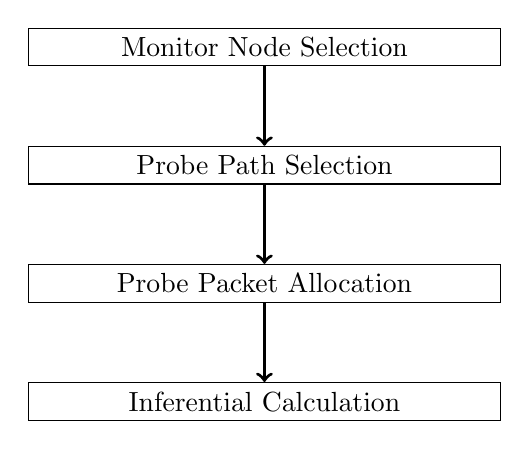
\begin{tikzpicture}
        \node[draw,minimum width=6cm] (A) at (0,4.5) {Monitor Node Selection};
        \node[draw,minimum width=6cm] (B) at (0,3) {Probe Path Selection};
        \node[draw,minimum width=6cm] (C) at (0,1.5) {Probe Packet Allocation};
        \node[draw,minimum width=6cm] (D) at (0,0) {Inferential Calculation};
        
        \draw[->, very thick] (A) -- (B);
        \draw[->, very thick] (B) -- (C);
        \draw[->, very thick] (C) -- (D);
    \end{tikzpicture}
    \caption{The Tomographic Pipeline.}
\end{figure}

\subsection{The Tomographic Pipeline}

\subsection{Parsimonious Probe Path Selection}
\label{ssec:Mpppselection}

\subsection{Probe Allocation}
\label{ssec:Mpallocation}

As probes traversing different nodes and different probes traversing the same node have an independent effect on $q$ we can develop an aggregation of all measurements in $\vec{q}$ assuming $r\in R, q_r \sim \mathcal{N}(0, \theta_r)$ where the variance $\theta_r$ is unknown. Using this this we aim to infer an estimation of $\vec{\theta}$ from our monitor-to-monitor measurements $\vec{q}$. To formalise our knowledge of the network from probing we adapt a standard PDV PMF from \cite{he_network_2021} where $\mathcal{M} = \sum_{r\in p}\theta_r$ in \cref{eq:pdvobservationmodel} and denote the corresponding log-likelihood function as $\widehat{\mathcal{L}}(q, p)$.
\begin{equation}
\label{eq:pdvobservationmodel}
    f_{Q|\vec{\theta},\; \vec{\phi}}(q,\;p) = \phi_p \sqrt{2\pi\mathcal{M}}^{\ q^2/{2\mathcal{M}_r}}
\end{equation}
Using $\widehat{\mathcal{L}}(q, p)$ we are able to represent a network as a FIM, from this the CRB can be posed as a metric representing the lower bound on the accuracy of our inference, we elaborate on the specifics of this representation in \cref{sec:Mnetworkprobing}. Using this CRB however we can show that the equal allocation of probes over paths is a sub optimal approach to probing. Consider the example network in \cref{fig:fimex3routereg} we define three probe paths $p_0$, $p_1$, and $p_3$ traversing $r_0\rightarrow r_2$, $\ r_1\rightarrow r_2$, $\ r_0\rightarrow r_1\rightarrow r_2$, and the reserve directions respectively.
\begin{figure}[H]
    \centering
    \tikzsetnextfilename{3routertopology}
    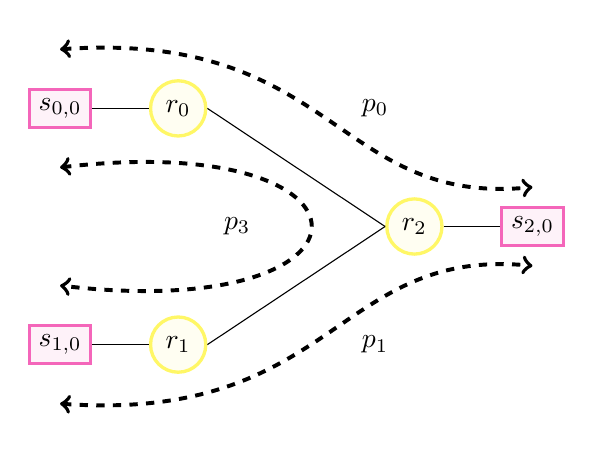
\begin{tikzpicture}[
        router/.style={circle, draw=yellow!60, fill=yellow!5, very thick, minimum size=3.5mm},
        nef_router/.style={circle, draw=red!60, fill=red!5, very thick, minimum size=3.5mm},
        switch/.style={rectangle, draw=cyan!60, fill=cyan!5, very thick, minimum size=2.5mm},
        monitor/.style={rectangle, draw=magenta!60, fill=magenta!5, very thick, minimum size=2.5mm},]
        
        % Routers
        \node[router] (r0) at (-1.5,1.5) {$r_0$};
        \node[router] (r1) at (-1.5,-1.5)  {$r_1$};
        \node[router] (r2) at (1.5,0) {$r_2$};
        %Switches
        \node[monitor](s00) at (-3,1.5)   {$s_{0,0}$};
        \node[monitor](s10) at (-3,-1.5)   {$s_{1,0}$};
        \node[monitor](s20) at (3,0)   {$s_{2,0}$};

        %Links
        \draw[-] (r0.east) -- (r2.west);
        \draw[-] (r1.east) -- (r2.west);
        \draw[-] (r0.west) -- (s00.east);
        \draw[-] (r1.west) -- (s10.east);
        \draw[-] (r2.east) -- (s20.west);
        
        % Probe path visualizations.
        \node at (1,1.5) {$p_0$};
        \draw[dashed, line width=.5mm, <->] (-3,2.25) .. controls (0.5,2.5) and (0.5,0.25) .. (3, 0.5);
        \node at (1,-1.5) {$p_1$};
        \draw[dashed, line width=.5mm, <->] (-3,-2.25) .. controls (0.5,-2.5) and (0.5,-0.25) .. (3, -0.5);
        \node at (-0.75,0) {$p_3$};
        \draw[dashed, line width=.5mm, <->] (-3,0.75) .. controls (1.25,1.25) and (1.25,-1.25) .. (-3, -0.75);

    \end{tikzpicture}
    \caption{Example 3 router network with probe paths explicitly noted.}
    \label{fig:fimex3routereg}
\end{figure}

We examine three different probe allocations between [$p_0,\:p_1$]: $\phi_0$ = [0.33, 0.33, 0.33],  $\phi_1$ = [0.1, 0.8, 0.1], and $\phi_2$ = [0.8, 0.1, 0.1]. As there are no nefarious routers each router has an equal expected true PDV, let these true PDV's be $r_0=1, r_1=1, r_2=1$, the CRB of each probe allocation is then $\phi_0$=2.69, $\phi_1$=5.97, $\phi_2$=5.97. Recalling that the CRB provides a lower bound on inferential accuracy, the equal allocation of probes between paths results in the lowest inferential accuracy, this also holds when nefarious behaviour is included. Suppose the case of $r_1$ being nefarious with a $\frac{1}{3}$ probability of holding a packet any timestep, resulting in an increased PDV of 3 the CRB of each probing scheme is then $\phi_0$=1.51, $\phi_1$=4.24, $\phi_2$=2.05. Although each probing scheme performs worse it is clear that $\phi_0$ is comparatively even worse at detecting the increased PDV of the nefarious router than the case of no nefarious nodes. Note for comparison that in the previous case of being $r_1$ nefarious a pseudo optimal probing allocation $\phi_{optimal}$ = [0.0, 0.5, 0.5] results in a CRB of 33.67.

\section{Evaluation Techniques}
\label{sec:Mevaltechniques}

\section{Summary}
\todo{Once chapter is finished recap what we showed with a reference to each section.}
